\section{基本群}
\sourcepage{244}
本节简要介绍同伦论，特别考察空间的基本群。同伦论的一个动机是识别并分类拓扑空间中的“洞”。圆环中心有洞，单位球面也有洞（图 4.10.1），但直觉上它们性质不同，或许具有不同维数。同伦论帮助我们整理这些想法。
\begin{center}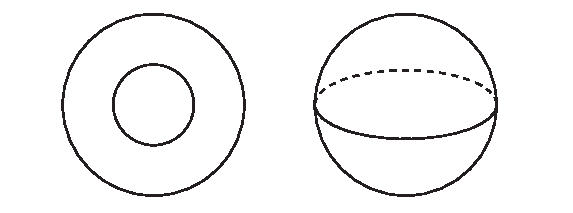
\includegraphics[width=.75\textwidth]{figures/4-10-1.pdf}\\图 4.10.1：不同类型的洞\end{center}
同伦论的出发点是空间 $X$ 中的所有\textbf{闭路}（loops）：即满足 $\gamma(0)=\gamma(1)$ 的连续映射 $\gamma:[0,1]\to X$。
\begin{center}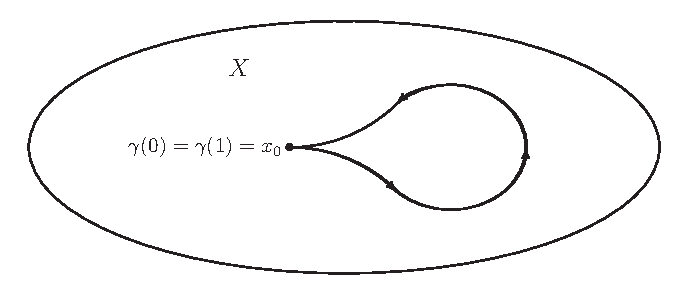
\includegraphics[width=.88\textwidth]{figures/4-10-2.pdf}\\图 4.10.2：$X$ 中的闭路\end{center}

\sourcepage{245}
\entry{定义}{4.10.1}固定 $x_0\in X$ 为\textbf{基点}（base point）。设 $\gamma_1,\gamma_2:[0,1]\to X$ 都以 $x_0$ 为起点和终点。若存在连续映射 $\Gamma:[0,1]\times[0,1]\to X$，满足
\begin{enumerate}[label=(\arabic*)]
\item $\Gamma(t,0)=\gamma_1(t)$，$0\le t\le1$；
\item $\Gamma(t,1)=\gamma_2(t)$，$0\le t\le1$；
\item $\Gamma(0,u)=x_0$，$0\le u\le1$；
\item $\Gamma(1,u)=x_0$，$0\le u\le1$，
\end{enumerate}
则称两闭路\textbf{保持基点同伦}（base-point homotopic），记为 $\gamma_1\simeq\gamma_2$，称 $\Gamma$ 为同伦映射。
\begin{center}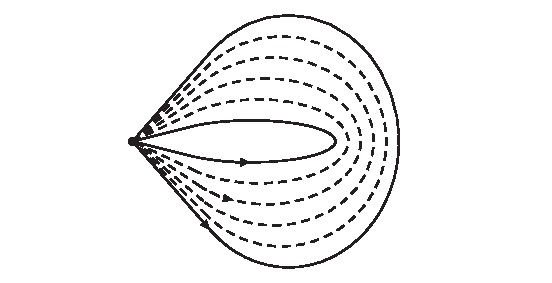
\includegraphics[width=.75\textwidth]{figures/4-10-3.pdf}\\图 4.10.3：两条同伦闭路\end{center}
图中还显示形变经过的一些中间闭路。图 4.10.4 则表示圆环中两条不能同伦的闭路；当然，“看起来不能同伦”还不等于证明它们不能同伦。

前两个条件说明它们作为映射同伦，后两个则要求形变中保持基点。因此这比定义 2.7.1 更强，但仍使用相同记号，由上下文区分。通常也简称“同伦”，不再提及基点。讨论和计算中，基点往往隐含不写。也有不固定基点的同伦理论，但这里介绍的是最常用的版本。

\sourcepage{246}
\begin{center}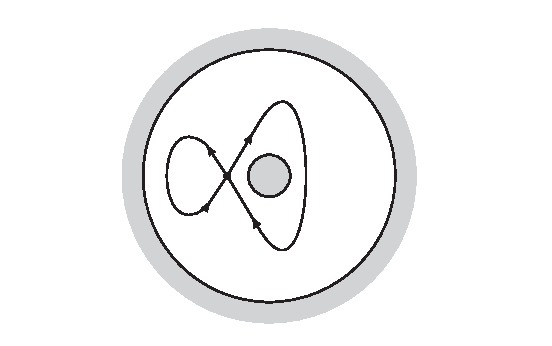
\includegraphics[width=.75\textwidth]{figures/4-10-4.pdf}\\图 4.10.4：圆环中两条不能同伦的闭路\end{center}
\entry{例}{4.10.2}设 $X$ 为欧氏空间的子集，$\gamma_1,\gamma_2$ 是具有同一基点的闭路。若对每个 $t$，从 $\gamma_1(t)$ 到 $\gamma_2(t)$ 的线段均在 $X$ 内，则
\[
\Gamma(t,u)=(1-u)\gamma_1(t)+u\gamma_2(t)
\]
给出保持基点的同伦。

\entry{引理}{4.10.3}定义 4.10.1 的关系在所有以 $x_0$ 为基点的闭路上是等价关系。

\textbf{证明：}自反性、对称性容易验证，只证传递性。若 $\Gamma_{12}$ 是从 $\gamma_1$ 到 $\gamma_2$ 的同伦，$\Gamma_{23}$ 是从 $\gamma_2$ 到 $\gamma_3$ 的同伦，令
\[
\Gamma_{13}(t,u)=\begin{cases}\Gamma_{12}(t,2u),&0\le u\le\tfrac12,\\\Gamma_{23}(t,2u-1),&\tfrac12\le u\le1.\end{cases}
\]
在接缝处两式都为 $\gamma_2(t)$，故映射良定义且连续。其端点值符合要求，给出从 $\gamma_1$ 到 $\gamma_3$ 的同伦。\hfill$\square$

\entry{定义}{4.10.4}闭路的等价类称为\textbf{同伦类}，$\gamma$ 的类记为 $[\gamma]$。这些类组成的集合称为第一同伦空间。定义乘积
\[
[\gamma]\cdot[\eta]=[\gamma\cdot\eta],\qquad
(\gamma\cdot\eta)(t)=\begin{cases}\gamma(2t),&0\le t\le\tfrac12,\\\eta(2t-1),&\tfrac12<t\le1.\end{cases}
\]
\sourcepage{247}
也就是说，先走 $\gamma$，再走 $\eta$，见图 4.10.5。下面将证明这使同伦类构成群，称为 $X$ 的\textbf{第一同伦群}或\textbf{基本群}（fundamental group），记为 $\pi_1(X,x_0)$，或简记 $\pi_1(X)$。我们采用乘法记号，单位元记为 $1$。
\begin{center}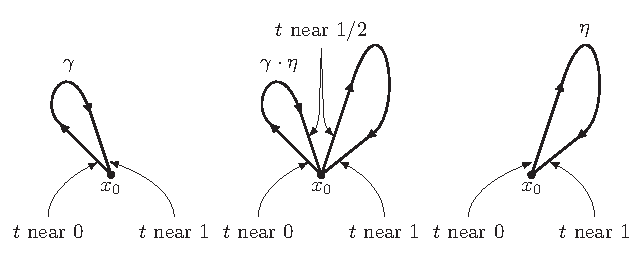
\includegraphics[width=.9\textwidth]{figures/4-10-5.pdf}\\图 4.10.5：$\gamma$ 与 $\eta$ 的乘积\end{center}

\entry{引理}{4.10.5}令 $\gamma_0(t)=x_0$ 为常值闭路，则：
\begin{enumerate}[label=(\arabic*)]
\item 上述乘法良定义；
\item 乘法满足结合律；
\item $[\gamma][\gamma_0]=[\gamma_0][\gamma]=[\gamma]$；
\item 若 $\eta(t)=\gamma(1-t)$，则 $[\gamma][\eta]=[\eta][\gamma]=[\gamma_0]$。
\end{enumerate}
\sourcepage{248}
\textbf{证明：}(1) 若 $\Gamma$ 给出 $\gamma\simeq\gamma'$，$\Phi$ 给出 $\eta\simeq\eta'$，则
\[
\Pi(t,u)=\begin{cases}\Gamma(2t,u),&0\le t\le\tfrac12,\ 0\le u\le1,\\\Phi(2t-1,u),&\tfrac12\le t\le1,\ 0\le u\le1\end{cases}
\]
是从 $\gamma\cdot\eta$ 到 $\gamma'\cdot\eta'$ 的同伦，见图 4.10.6。\translatornote{原书第二行把 $u$ 的上限误印为 $1/2$，应为 $1$。}其余三点也容易，留作习题。\hfill$\square$
\begin{center}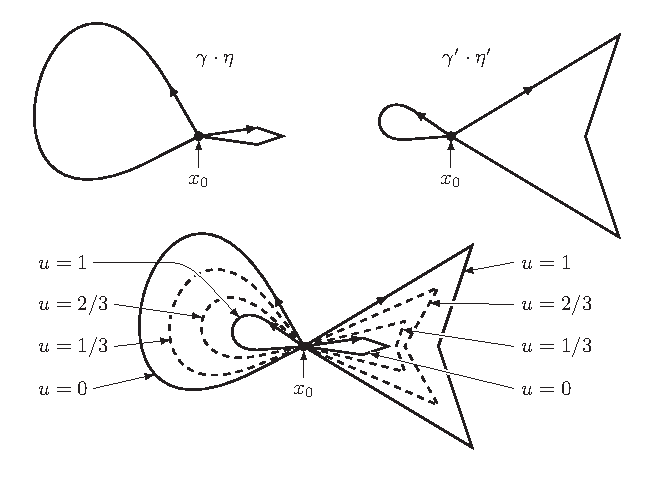
\includegraphics[width=.88\textwidth]{figures/4-10-6.pdf}\\图 4.10.6：乘积闭路间的同伦\end{center}
因此这确实是同伦类集合上的群运算。还有高阶同伦群 $\pi_k(X)$，但本书此处不讨论。基本群的重要性质是函子性。

\entry{定理}{4.10.6}若 $f:X\to Y$ 连续且 $f(x_0)=y_0$，则
\[
f_*:\pi_1(X,x_0)\to\pi_1(Y,y_0),\qquad f_*[\gamma]=[f\circ\gamma]
\]
是群同态。

\sourcepage{249}
\textbf{证明：}若 $\Gamma$ 是两闭路间的同伦，则 $f\circ\Gamma$ 是复合闭路间的同伦，所以良定义。又由分段定义，
\[
f\circ(\gamma\cdot\eta)=(f\circ\gamma)\cdot(f\circ\eta),
\]
故 $f_*([\gamma][\eta])=f_*[\gamma]f_*[\eta]$。\hfill$\square$

原书接着声称：“若 $f$ 单射，则 $f_*$ 单射；若 $f$ 满射，则 $f_*$ 满射。”\translatornote{这两句话一般都不成立。例如包含 $S^1\hookrightarrow B^2$ 是单射，却在基本群上诱导 $\Z\to0$；满射 $[0,1]\to S^1$，$t\mapsto e^{2\pi it}$，在基本群上诱导 $0\to\Z$。下面的拓扑不变性应由恒等与复合的函子性质，以及同胚的逆映射推出。}

\entry{推论}{4.10.7}基本群是空间的拓扑不变量。

因此同胚空间有同构的基本群；基本群不同构的空间不可能同胚。回忆单纯同调的定义与拓扑不变性证明曾需要很多准备，而基本群在几页之内就定义并证明了不变性。不过，计算基本群时，同伦论就变得更具挑战。

\entry{命题}{4.10.8}圆周的基本群同构于整数群：$\pi_1(S^1)\cong\Z$。

\textbf{证明：}把 $S^1$ 视为 $\{z\in\mathbb C:|z|=1\}$，基点取 $1$，记 $I=[0,1]$。闭路 $\sigma:I\to S^1$ 满足 $\sigma(0)=\sigma(1)=1$。令
\[
\varphi:\R\to S^1,\quad\varphi(x)=e^{2\pi ix},\qquad
\rho_n(t)=\varphi(nt)=e^{2\pi int}\quad(n\in\Z).
\]
若 $n>0$，$\rho_n$ 逆时针绕圆周 $n$ 圈；若 $n<0$，顺时针绕 $|n|$ 圈；$\rho_0$ 为常值闭路。

\sourcepage{250}
先证明每条 $\sigma$ 都同伦于某个 $\rho_n$。希望找到连续映射 $\sigma':I\to\R$，满足 $\sigma=\varphi\sigma'$、$\sigma'(0)=0$。于是 $\sigma'(1)=n\in\Z$，而
\[
\Gamma(t,u)=\varphi\bigl((1-u)\sigma'(t)+unt\bigr)
\]
就是从 $\sigma$ 到 $\rho_n$ 的同伦。称 $\sigma'$ 为 $\sigma$ 的\textbf{提升}（lifting），即使 $\varphi\sigma'=\sigma$ 的图交换。

形式上，似乎可以令 $\sigma'(t)=(2\pi i)^{-1}\log\sigma(t)$，但闭路通常绕遍圆周，无法全局使用单值对数。诀窍是：$\varphi$ 将 $(-1/2,1/2)$ 同胚地映到 $S^1\setminus\{-1\}$，其逆在这个集合上良定义。

由 $\sigma$ 在紧区间上的一致连续性，可取 $\varepsilon>0$，使 $|t-t'|<\varepsilon$ 时 $|\sigma(t)-\sigma(t')|<1$，于是 $\sigma(t)/\sigma(t')\ne-1$。\translatornote{原书在本段一致连续性的主语处两次误写为 $\varphi$，此处实际用的是 $\sigma$。}取 $K$ 使 $1/K<\varepsilon$，令 $p_i=i/K$，定义
\[
\sigma'(t)=\sum_{i=0}^{K-1}\varphi^{-1}\left(\frac{\sigma(tp_{i+1})}{\sigma(tp_i)}\right).
\]
各项因 $|tp_{i+1}-tp_i|<\varepsilon$ 而有意义，且连续。指数把和变为积，所以
\[
\varphi(\sigma'(t))=\prod_{i=0}^{K-1}\frac{\sigma(tp_{i+1})}{\sigma(tp_i)}
=\frac{\sigma(tp_K)}{\sigma(tp_0)}=\sigma(t).
\]

\sourcepage{251}
同样可提升同伦 $F:I\times I\to S^1$。取一致连续性参数 $\varepsilon$，令 $1/K<\varepsilon/2$，定义
\[
F'(t,u)=\sum_{i=0}^{K-1}\varphi^{-1}\left(\frac{F(tp_{i+1},up_{i+1})}{F(tp_i,up_i)}\right).
\]
因为
\[
\|(tp_{i+1},up_{i+1})-(tp_i,up_i)\|
\le |u(p_{i+1}-p_i)|+|t(p_{i+1}-p_i)|<\varepsilon,
\]
公式有意义，且 $\varphi F'=F$。若 $F$ 连接 $\rho_m$ 与 $\rho_n$，则 $F'(1,0)=m$、$F'(1,1)=n$。函数 $F'(1,u)$ 连续且取整数值，故为常值，得 $m=n$。因此各 $[\rho_n]$ 不同。最后验证 $[\rho_m][\rho_n]=[\rho_{m+n}]$ 即完成证明，这一步留作习题。\hfill$\square$

\entry{例}{4.10.9}若 $X$ 同胚于欧氏空间的凸子集，则 $\pi_1(X)=1$。由拓扑不变性，可设 $X$ 本身凸。固定基点 $x_0$，任一闭路与常值闭路由例 4.10.2 的线性同伦连接，故所有类都是单位元。这里用 $1$ 而非 $\{1\}$ 简记平凡乘法群。

若 $\pi_1(X)=1$，本书称 $X$ \textbf{单连通}（simply connected）。

\entry{例}{4.10.10}当 $n\ge2$ 时，$\pi_1(S^n)=1$。以 $n=2$ 为例。不能直接断言每条闭路的像包含于同胚于平面圆盘的球面子集：Peano 于 1890 年构造了空间填充曲线，闭路的像甚至可能覆盖整个球面。\footnote{原论文为 [Pea90]；Hilbert 在 [Hil91] 中给出了有帮助的图。英文说明见 [Mun00] 第 44 节。}不过，总可通过同伦修改闭路，使新闭路包含于这样的子集中。细节留作习题。

\sourcepage{252}
\subsection*{与同调的关系}
回忆奇异 $p$ 维单形是 $T:\Delta_p\to X$，其中 $\Delta_p$ 是 $\R^\infty$ 中顶点为 $\epsilon_0=0,\epsilon_1,\ldots,\epsilon_p$ 的标准单形。本小节只涉及不超过二维的单形，因此改在有限维空间中取
\[
\Delta_2=\operatorname{conv}\{(0,0),(1,0),(0,1)\},\quad\Delta_1=[0,1],\quad\Delta_0=\{0\}.
\]
\translatornote{原书将三角形的第三个顶点印为 $(1,1)$；后面所有边缘公式和证明实际使用的是 $(0,1)$。}奇异单形仍是从相应三角形、区间或单点到 $X$ 的连续映射，边缘为
\[
\partial T=\begin{cases}0,&T\text{ 为零维单形},\\T(1)-T(0),&T\text{ 为一维单形},\\S_0-S_1+S_2,&T\text{ 为二维单形},\end{cases}
\]
其中 $S_0(t)=T(1-t,t)$、$S_1(t)=T(0,t)$、$S_2(t)=T(t,0)$。读者应核对它与第 4.2 节的定义一致。常值一维单形既是闭链，也是同值的常值二维单形的边缘。

同伦概念也适用于一般道路，而不限于闭路。

\sourcepage{253}
\entry{定义}{4.10.11}设 $a<b$，$p_1,p_2:[a,b]\to X$ 有相同起点和终点。若存在同伦 $F:[a,b]\times I\to X$，满足
\[
F(t,0)=p_1(t),\quad F(t,1)=p_2(t),\quad
F(a,u)=p_1(a)=p_2(a),\quad F(b,u)=p_1(b)=p_2(b),
\]
则称两道路\textbf{保持端点同伦}，记为 $p_1\simeq p_2\ \operatorname{rel}\{a,b\}$。

\entry{引理}{4.10.12}设 $x,y\in X$。
\begin{enumerate}[label=(\arabic*)]
\item 若奇异一维单形 $p$ 满足 $\partial p=y-x$，且 $p^{-1}(t)=p(1-t)$，则 $p+p^{-1}$ 是边缘。
\item 若 $p_1,p_2$ 满足 $\partial p_i=y-x$，且保持端点同伦，则它们同调。
\end{enumerate}
\textbf{证明：}(1) 令 $T(t,u)=p(1-t)$。三条边为 $S_0(t)=p(t)$、$S_1(t)=y$、$S_2(t)=p(1-t)$。故 $\partial T=p-y+p^{-1}$；而常值一维单形 $y$ 也是边缘，结论成立。

(2) 设 $F$ 是从 $p_1$ 到 $p_2$ 的端点固定同伦。定义 $T(t,u)=F(t,u)$，则其边为
\[
S_0(t)=F(1-t,t),\quad S_1(t)=x,\quad S_2(t)=p_1(t).
\]
再定义 $T'(t,u)=F(t+u,1-t)$，则
\[
S'_0(t)=y,\quad S'_1(t)=p_2(t),\quad S'_2(t)=F(t,1-t).
\]
令 $p(t)=F(1-t,t)$，有 $\partial(T+T')=p_1-p_2+y-x+p+p^{-1}$。常值链 $x,y$ 及 $p+p^{-1}$ 均为边缘，故 $p_1-p_2$ 为边缘。\hfill$\square$

\sourcepage{254}
\entry{定义}{4.10.13}每条以 $x_0$ 为基点的闭路也是奇异一维闭链，因为 $\partial\gamma=x_0-x_0=0$。其同调类记为 $\{\gamma\}$。定义
\[
\chi:\pi_1(X,x_0)\to H_1(X),\qquad\chi([\gamma])=\{\gamma\}.
\]
由上一个引理，此映射良定义。

\entry{定义}{4.10.14}在乘法群 $G$ 中，$a^{-1}b^{-1}ab$ 称为 $a,b$ 的\textbf{换位子}（commutator）。所有换位子生成的子群称为\textbf{换位子子群}（commutator subgroup）。

\entry{定理}{4.10.15}设 $X$ 为拓扑空间，$x_0$ 为基点。
\begin{enumerate}[label=(\arabic*)]
\item $\chi:\pi_1(X,x_0)\to H_1(X)$ 为群同态。
\item 若 $X$ 道路连通，$\chi$ 满射。
\item 若 $X$ 道路连通，$\ker\chi$ 是基本群的换位子子群。
\item 若 $X$ 道路连通，$\chi$ 为同构当且仅当基本群交换。
\end{enumerate}
因此若换位子子群为 $C$，则 $\pi_1(X,x_0)/C\cong H_1(X)$。这就是第一同调群是第一同伦群的\textbf{阿贝尔化}（abelianization）的含义。

先证明一个把道路分成小段的引理。

\sourcepage{255}
\entry{引理}{4.10.16}设 $0=a_0<a_1<\cdots<a_r=1$，$T:[0,1]\to X$ 为奇异一维单形。则 $T$ 同调于 $\sum_{i=0}^{r-1}T_i$，其中 $T_i(t)=T((1-t)a_i+ta_{i+1})$。
\begin{center}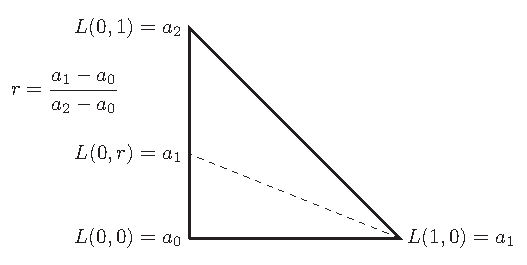
\includegraphics[width=.72\textwidth]{figures/4-10-7.pdf}\\图 4.10.7\end{center}
\textbf{证明：}只需考虑二等分情形 $r=2$。取仿射函数 $L(x,y)=a_0+(a_1-a_0)x+(a_2-a_0)y$，其顶点值如图所示。令 $W=T\circ L$。其三条边分别是 $T_1,T,T_0$，故 $\partial W=T_1-T+T_0$，即 $T$ 同调于 $T_0+T_1$。\translatornote{原书证明末句把这两个分段链误写为 $T_1+T_2$。}\hfill$\square$

\textbf{定理 4.10.15 的证明：}(1) 要证 $\chi([\gamma\cdot\gamma'])=\chi[\gamma]+\chi[\gamma']$。由上一个引理，乘积道路作为奇异单形同调于链 $\gamma+\gamma'$，即得结论。

(2) 假设 $X$ 道路连通。对每个 $x\in X$，选道路 $\zeta_x$ 从 $x_0$ 到 $x$，取 $\zeta_{x_0}$ 为常值道路；其逆向道路为 $\zeta_x^{-1}(t)=\zeta_x(1-t)$。

\sourcepage{256}
给定奇异一维闭链 $z=\sum n_i\sigma_i$，构造闭路
\[
\gamma_i(t)=\begin{cases}
\zeta_{\sigma_i(0)}(3t),&0\le t\le\tfrac13,\\
\sigma_i(3t-1),&\tfrac13\le t\le\tfrac23,\\
\zeta_{\sigma_i(1)}^{-1}(3t-2),&\tfrac23\le t\le1.
\end{cases}
\]
由 (1) 及分段引理，
\[
\chi\left(\prod_i[\gamma_i]^{n_i}\right)
=\sum_i n_i\{\gamma_i\}
=\left\{\sum_i n_i(\zeta_{\sigma_i(0)}-\zeta_{\sigma_i(1)})+z\right\}.
\]
由于 $z$ 闭，$\sum n_i(\sigma_i(1)-\sigma_i(0))=0$。对其中每个端点 $x$，其总系数为零；将同一点换成预先固定的道路 $\zeta_x$，总系数仍为零。因此上式的道路项抵消，结果恰为 $\{z\}$，证明满射。

(3) 记换位子子群为 $C$。因为 $H_1(X)$ 交换，$\chi$ 将每个换位子映为零，故 $C\subset\ker\chi$。商群 $\pi_1/C$ 为交换群，这将允许我们交换并合并各项。

\sourcepage{257}
若 $[\gamma]\in\ker\chi$，则作为奇异链有 $\gamma=\partial(\sum n_i\sigma_i)$，其中 $\sigma_i$ 为二维单形。记
\[
\alpha_{i0}(t)=\sigma_i(1-t,t),\quad\alpha_{i1}(t)=\sigma_i(0,t),\quad\alpha_{i2}(t)=\sigma_i(t,0),
\]
则
\[
\gamma=\sum_i n_i(\alpha_{i0}-\alpha_{i1}+\alpha_{i2}).\tag{$\dagger$}
\]
这是真正的链相等，而不只是同调；合并相同道路后，$\gamma$ 的系数为 $1$，其他道路系数为零。
\begin{center}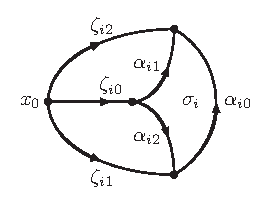
\includegraphics[width=.43\textwidth]{figures/4-10-8.pdf}\\图 4.10.8：单形、各边及从基点到顶点的道路\end{center}
记三个顶点为
\begin{align*}
x_{i0}&=\sigma_i(0,0)=\alpha_{i1}(0)=\alpha_{i2}(0),\\
x_{i1}&=\sigma_i(1,0)=\alpha_{i0}(0)=\alpha_{i2}(1),\\
x_{i2}&=\sigma_i(0,1)=\alpha_{i0}(1)=\alpha_{i1}(1).
\end{align*}
简记 $\zeta_{ij}=\zeta_{x_{ij}}$。将各边补成以 $x_0$ 为基点的闭路：
\[
\beta_{i0}=\zeta_{i1}\cdot\alpha_{i0}\cdot\zeta_{i2}^{-1},\quad
\beta_{i1}=\zeta_{i0}\cdot\alpha_{i1}\cdot\zeta_{i2}^{-1},\quad
\beta_{i2}=\zeta_{i0}\cdot\alpha_{i2}\cdot\zeta_{i1}^{-1}.
\]
道路乘积从左到右依次行走，并适当重参数化为 $[0,1]$ 上的映射，相当于分段引理的逆过程。

\sourcepage{258}
\begin{center}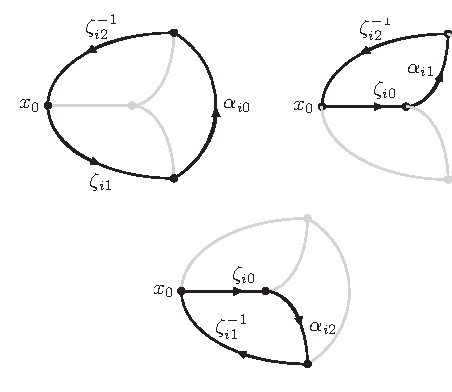
\includegraphics[width=.7\textwidth]{figures/4-10-9.pdf}\\图 4.10.9：三个补成的闭路\end{center}
令 $\beta_i=\beta_{i0}\cdot\beta_{i1}^{-1}\cdot\beta_{i2}$。展开后，成对的道路及其逆可通过保持端点的同伦消去，得
\begin{align*}
\beta_i
&=\zeta_{i1}\cdot\alpha_{i0}\cdot\zeta_{i2}^{-1}\cdot
(\zeta_{i0}\cdot\alpha_{i1}\cdot\zeta_{i2}^{-1})^{-1}\cdot
\zeta_{i0}\cdot\alpha_{i2}\cdot\zeta_{i1}^{-1}\\
&\simeq\zeta_{i1}\cdot\alpha_{i0}\cdot\alpha_{i1}^{-1}\cdot\alpha_{i2}\cdot\zeta_{i1}^{-1}.
\end{align*}
\begin{center}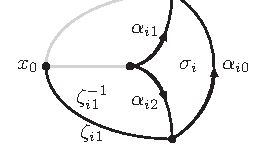
\includegraphics[width=.43\textwidth]{figures/4-10-10.pdf}\\图 4.10.10：闭路 $\beta_i$\end{center}
它从基点走到 $x_{i1}$，绕单形边缘一周，再原路返回。将 $\Delta_2$ 收缩到 $(1,0)$，便将绕边缘的部分收缩到 $x_{i1}$。所以 $\beta_i\simeq\zeta_{i1}\cdot\zeta_{i1}^{-1}\simeq x_0$，即 $[\beta_i]=1$，因而
\[
\prod_i[\beta_i]^{n_i}=1.\tag{$\ddagger$}
\]

\sourcepage{259}
若基本群交换，就可像 ($\dagger$) 那样合并道路项；一般基本群不交换，不能这样做。但在交换商群 $\pi_1/C$ 中可以。记闭路 $\beta$ 的陪集为 $\lceil\beta\rceil$。由 ($\ddagger$)，有 $\prod_i\lceil\beta_i\rceil^{n_i}=1$；而由 ($\dagger$)，把每条边按上述相同规则补成闭路后，所有同一道路的项仍抵消，所得积等于 $\lceil\gamma\rceil$。因此 $\lceil\gamma\rceil=1$，即 $[\gamma]\in C$。这证明 $\ker\chi=C$。

(4) 由 (2)、(3) 立即得到。\hfill$\square$

\begin{center}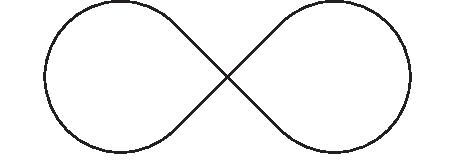
\includegraphics[width=.65\textwidth]{figures/4-10-11.pdf}\\图 4.10.11：数字 8 空间\end{center}
\entry{命题}{4.10.17}图 4.10.11 的数字 8 空间 $X$ 的基本群不是阿贝尔群。

\textbf{证明：}仍把圆周视为复数单位圆，并将 $X$ 视为 $(S^1\times\{1\})\cup(\{1\}\times S^1)$，基点为 $(1,1)$。这个模型位于两个平面的笛卡儿积中：两个圆周只在基点相交。

\sourcepage{260}
令 $\gamma(t)=(e^{2\pi it},1)$、$\eta(t)=(1,e^{2\pi it})$，其逆向闭路分别把 $t$ 换为 $1-t$。令 $\zeta=\gamma\cdot\eta\cdot\gamma^{-1}\cdot\eta^{-1}$。它依次逆时针绕第一、第二圆周，再顺时针绕第一、第二圆周。

反设基本群交换，则 $[\zeta]=1$，存在 $F:I\times I\to X$，使 $F(t,0)=F(0,u)=F(1,u)=(1,1)$，$F(t,1)=\zeta(t)$。定义
\[
\varphi:(\R\times\Z)\cup(\Z\times\R)\to X,\qquad
\varphi(w,z)=(e^{2\pi iw},e^{2\pi iz}).
\]
仿照命题 4.10.8，分别对两坐标作提升，可得 $\zeta'$ 与 $F'$，满足 $\varphi\zeta'=\zeta$、$\varphi F'=F$。由于至少有一个指数坐标为 $1$，提升的像确实在上述整数网格中。$\zeta'$ 正是沿单位正方形边缘逆时针绕一周的闭路。

再定义 $\psi$：从正方形中心 $(1/2,1/2)$ 作射线，经网格点 $(x,y)$，取它与 $\Bd(I\times I)$ 的唯一交点作为 $\psi(x,y)$，见图 4.10.12。它在正方形边缘上为恒等映射。\translatornote{原书用从 $(x,y)$ 到中心的线段与边缘的交点描述此映射；网格点没有落在正方形内部，故该描述给出相同的径向投影。}

于是 $\psi\zeta'$ 绕正方形边缘一周。因该边缘同胚于圆周，命题 4.10.8 说明此闭路不可能同伦于常值闭路；但 $\psi F'$ 恰给出它与常值 $(0,0)$ 的同伦，矛盾。\hfill$\square$

\sourcepage{261}
\begin{center}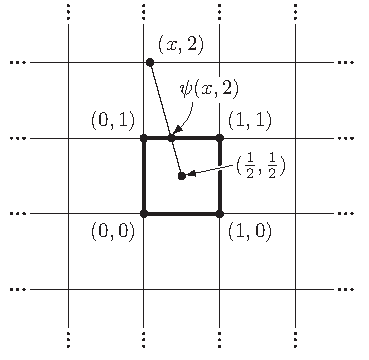
\includegraphics[width=.55\textwidth]{figures/4-10-12.pdf}\\图 4.10.12：映射 $\psi$\end{center}
\subsection*{习题}
\begin{enumerate}
\item 证明定义 4.10.1 的关系具有自反性、对称性。
\item 证明引理 4.10.5 的 (2)、(3)、(4)。
\item 参照命题 4.10.8 的证明，验证 $[\rho_m][\rho_n]=[\rho_{m+n}]$。
\item \begin{enumerate}[label=(\alph*)]
\item 证明 $n\ge2$ 时，$\R^n$ 中每条闭路均同伦于包含在有限条直线之并中的闭路。
\item 证明 $n\ge2$ 时，$S^n$ 中每条闭路均同伦于包含在有限条大圆之并中的闭路。这就验证了例 4.10.10 中的断言。\translatornote{原书将这里引用的例号印为 4.10.9。}
\end{enumerate}
\item 设 $X=U\cup V$，其中 $U,V$ 是单连通开集。若 $U\cap V$ 道路连通，证明 $X$ 单连通。
\end{enumerate}
